We evaluated two multi-agent oracle architectures on 1,189 resolved prediction market questions from KalshiBench. Three LLMs served as oracle agents: GPT-5 Nano, DeepSeek-V3, and 
Llama-3.3-70B. All agents received identical retrieved evidence for each question, isolating reasoning capability from retrieval quality. Architecture A (Independent Aggregation) has each model resolve independently, with outcomes determined by majority vote or confidence-weighted vote. Architecture B (Deliberative Consensus) has models engage in structured debate over two rounds, viewing each other's reasoning before submitting final answers.

\subsection{Overall Accuracy: Independent Aggregation Outperforms Both Single-Model Baselines and Deliberative Consensus}

\begin{table}[t]
\centering
\begin{tabular}{llc}
\toprule
\textbf{Group} & \textbf{System} & \textbf{Accuracy (\%)} \\
\midrule
\multirow{3}{*}{Single-LLM Baselines}
    & GPT-4o          & 82.34 \\
    & DeepSeek        & 82.42 \\
    & Llama           & 81.24 \\
\midrule
\multirow{2}{*}{Architecture A}
    & Majority Vote            & 82.93 \\
    & \textbf{Confidence-Weighted Vote} & \textbf{83.43} \\
\midrule
\multirow{4}{*}{Architecture B}
    & Final-Round GPT-4o       & 74.35 \\
    & Final-Round DeepSeek     & 76.70 \\
    & Final-Round Llama        & 76.37 \\
    & Deliberative Final       & 76.11 \\
\midrule
Prior Work (KalshiBench)
    & Claude Opus 4.5          & 69.3 \\
\bottomrule
\end{tabular}
\caption{Overall resolution accuracy across all 1,189 questions.}
\label{tab:overall}
\end{table}

Table~\ref{tab:overall} presents overall resolution accuracy across all 1,189 questions. Architecture A's confidence-weighted vote achieves the highest accuracy at 83.43\%, representing a +1.01 percentage point improvement over the best individual model (DeepSeek, 82.42\%). Majority voting also outperforms every single-model baseline at 82.93\%. Architecture B's deliberative process, by contrast, \emph{degrades} performance substantially: all final-round outputs fall below every single-model baseline, with the best deliberative result (Final-Round DeepSeek, 76.70\%) trailing the worst individual model (Llama, 81.24\%) by over four percentage points. As shown in Figure~\ref{fig:overall_accuracy}, independent aggregation consistently outperforms both single-model baselines and deliberative consensus.

\begin{figure}[t]
\centering
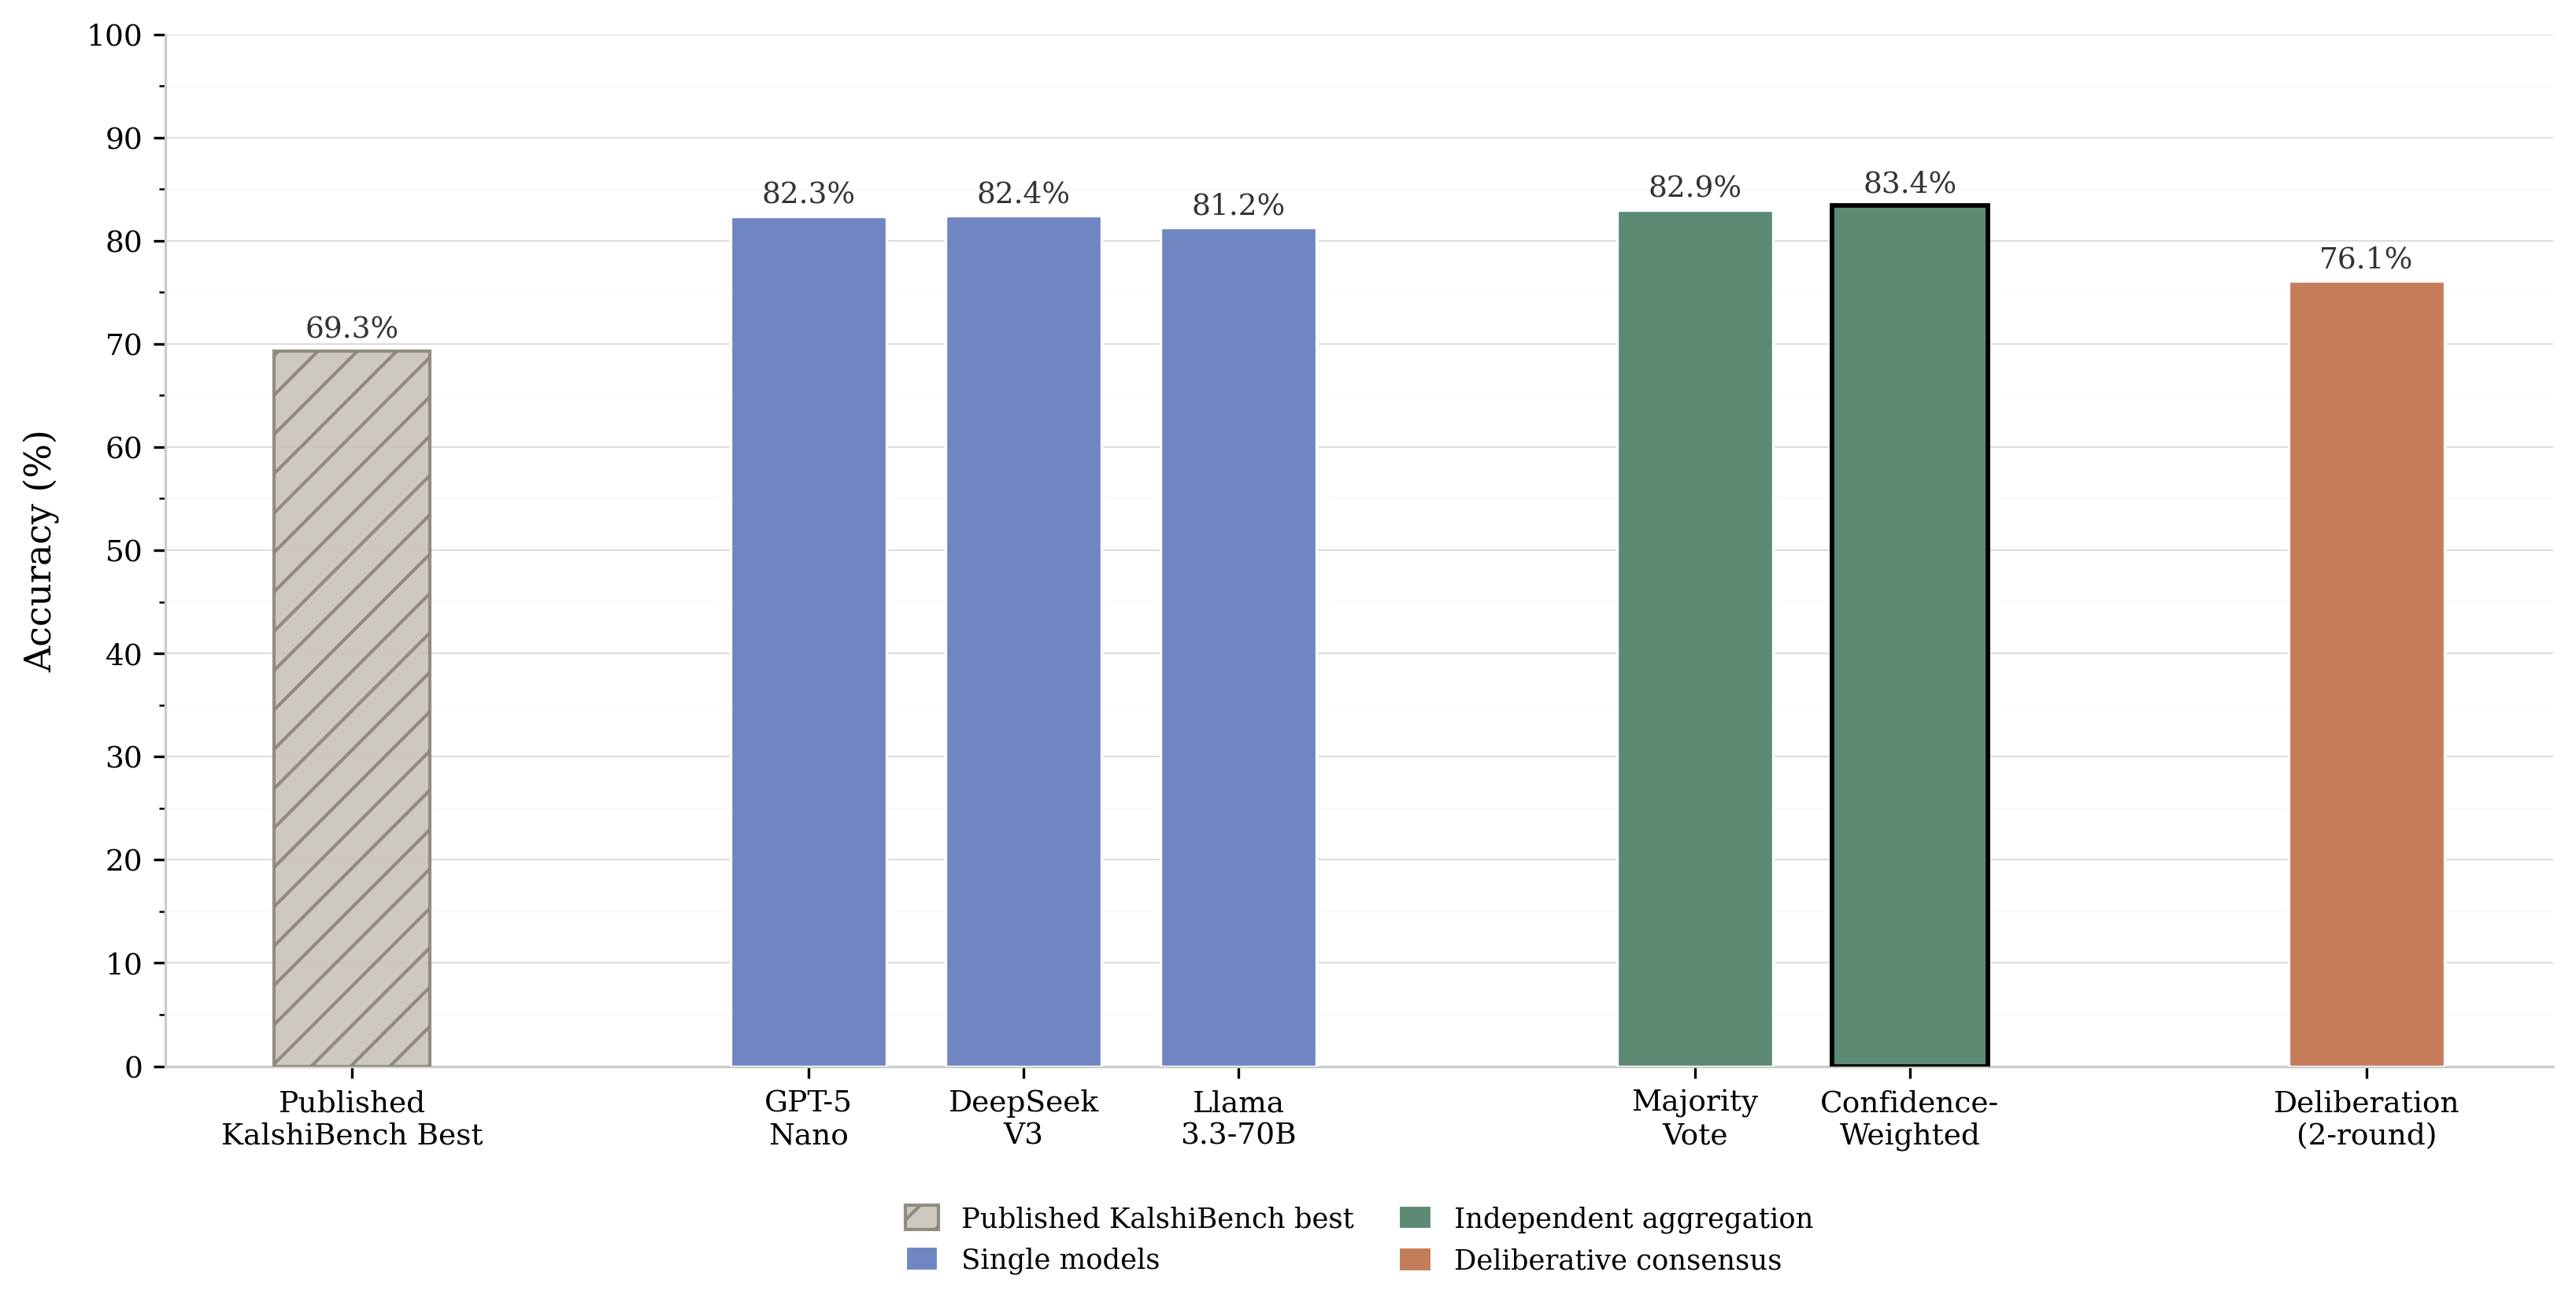
\includegraphics[width=\linewidth]{figures/figure3_overall_accuracy.png}
\caption{\textbf{Overall resolution accuracy on 1,189 KalshiBench questions.} Confidence-weighted independent aggregation (Architecture A) achieves the highest accuracy at 83.43\%, outperforming the best single-model baseline by 1.01 percentage points. Deliberative consensus (Architecture B) degrades accuracy to 76.11\%, below all single-model baselines. The hatched bar shows the best previously published KalshiBench result}
\label{fig:overall_accuracy}
\end{figure}

All systems substantially outperform the best previously reported result on KalshiBench, Claude Opus 4.5 at 69.3\%, though this comparison should be interpreted cautiously, as our pipeline uses a different retrieval layer (Exa with date-filtered evidence) than the original KalshiBench evaluation (which relied on the Model's general web search API). The improvement likely reflects the combined effect of better retrieval and multi-agent reasoning rather than model superiority alone.

To confirm that Architecture A's advantage over Architecture B is not an artifact of variance, we conducted McNemar's test for paired differences and a head-to-head comparison on the 1,170 overlapping questions evaluated by both architectures (Table~\ref{tab:mcnemar} and Table~\ref{tab:h2h}).

\begin{table}[t]
\centering
\caption{McNemar's test for paired accuracy differences. Each row compares two systems on the same question set. ``A only'' and ``B only'' indicate the number of questions each system answered correctly that the other missed. Significant results ($p < 0.05$) are bolded.}
\label{tab:mcnemar}
\begin{tabular}{llcccc}
\toprule
\textbf{System A} & \textbf{System B} & \textbf{A only} & \textbf{B only} & \textbf{Discordant} & $p$\textbf{-value} \\
\midrule
A Majority & A Weighted & 1 & 7 & 8 & 0.070 \\
\textbf{A Majority} & \textbf{B Deliberative} & \textbf{117} & \textbf{37} & \textbf{154} & $\mathbf{7.2 \times 10^{-11}}$ \\
\textbf{A Weighted} & \textbf{B Deliberative} & \textbf{123} & \textbf{37} & \textbf{160} & $\mathbf{5.5 \times 10^{-12}}$ \\
\bottomrule
\end{tabular}
\end{table}

Architecture A significantly outperforms Architecture B ($p < 10^{-10}$), and the asymmetry is stark: Architecture A correctly resolves 117 questions that B gets wrong, while B captures only 37 that A misses, a roughly 3:1 ratio. Within Architecture A, the difference between majority and confidence-weighted voting is not statistically significant ($p = 0.07$), though weighted voting trends better by picking up 7 additional correct resolutions at the cost of only 1.

\begin{table}[t]
\centering
\caption{Head-to-head comparison between Architecture A (confidence-weighted vote) and Architecture B (deliberative final) on the $n = 1{,}170$ overlapping questions evaluated by both systems. ``A correct, B wrong'' indicates questions where only independent aggregation produced the correct resolution.}
\label{tab:h2h}
\begin{tabular}{lc}
\toprule
\textbf{Outcome} & \textbf{Count (\%)} \\
\midrule
Both correct       & 852 (72.8\%) \\
A correct, B wrong & 117 (10.0\%) \\
B correct, A wrong &  37 (3.2\%) \\
Both wrong         & 164 (14.0\%) \\
\midrule
Architecture A accuracy & 82.8\% \\
Architecture B accuracy & 76.0\% \\
\bottomrule
\end{tabular}
\end{table}

The 164 questions (14.0\%) wrong under both architectures represent a ``hard core'' of failures that multi-agent reasoning alone cannot resolve. These questions likely require either higher-quality evidence retrieval or human judgment, a finding we revisit in the Escalation Analysis (Section~\ref{sec:escalation}).

\subsubsection{Robustness Check: Unique-Market Accuracy and Multi-Instance Consistency}

Because KalshiBench contains multi-instance markets, where a single market (e.g., ``Which company will IPO in 2026?'') is decomposed into multiple binary rows, one per possible outcome (e.g., ``Did Stripe IPO in 2026?'', ``Did Klarna IPO in 2026?''), the 1,189 rows correspond to only 703 unique markets. Of these, 486 markets appear in more than one row. To ensure our headline results are not inflated by over-counting repeated instances, we also evaluated accuracy at the unique-market level, keeping one row per \texttt{question\_id}. Architecture A achieves 81.9\% accuracy on unique markets (95\% Wilson CI: [0.789, 0.846]), and Architecture B achieves 75.5\% (95\% Wilson CI: [0.722, 0.786]). These numbers are consistent with the full-dataset results, confirming that the accuracy gap between architectures is not an artifact of repeated market weighting.

The multi-instance markets also reveal an important finding about resolution \emph{consistency}. For these 486 markets, each architecture resolves multiple binary outcomes drawn from the same parent market with the same retrieved evidence. Table~\ref{tab:consistency} shows how often each architecture produces consistent outcomes across all instances of a given market.

\begin{table}[t]
\centering
\caption{Resolution consistency across 486 multi-instance markets (markets with more than one binary outcome row in the dataset). ``All correct'' means every outcome for that market was resolved correctly. ``Mixed'' means at least one outcome was correct and at least one was incorrect within the same market, despite shared underlying evidence. ``All incorrect'' means every outcome was resolved incorrectly.}
\label{tab:consistency}
\begin{tabular}{lccc}
\toprule
\textbf{Architecture} & \textbf{All Correct} & \textbf{Mixed} & \textbf{All Incorrect} \\
\midrule
A (Independent)  & 380 (78.2\%) & 67 (13.8\%) & 39 (8.0\%) \\
B (Deliberative) & 338 (69.5\%) & 90 (18.5\%) & 58 (11.9\%) \\
\bottomrule
\end{tabular}
\end{table}

Architecture A resolves all outcomes correctly for 78.2\% of multi-instance markets compared to 69.5\% for Architecture B. More notably, Architecture B produces mixed-consistency outcomes on 90 markets (18.5\%) versus 67 (13.8\%) for Architecture A. These mixed cases are particularly concerning for oracle design: given the same parent market and the same retrieved evidence, the system correctly resolves some outcomes but not others. In a deployed oracle, this inconsistency could create exploitable discrepancies across related contracts within the same market. The finding suggests that deliberation not only reduces accuracy but also introduces additional variance into the resolution process, likely because the multi-round debate amplifies sensitivity to how individual outcomes within a market are framed.

These results partially align with prior multi-agent literature. The Iterative Consensus Ensemble (ICE) framework reported 7--15 percentage point improvements from multi-agent aggregation on medical reasoning benchmarks~\cite{omar2025ice}. Our independent aggregation gains are more modest (+1.01 pp), likely because our single-model baselines already achieve over 82\% accuracy, leaving less room for improvement. More critically, our deliberation architecture reduces accuracy, the opposite of what Du et al.~\cite{du2023debate} found for arithmetic tasks, where three-agent debate improved accuracy from roughly 70\% to 95\%. The difference likely reflects the nature of oracle resolution: unlike arithmetic where a correct derivation can be verified step-by-step, prediction market outcomes depend on evidence interpretation where confident-sounding but incorrect reasoning can be persuasive enough to flip correct initial judgments, a dynamic we analyze in Section~\ref{sec:errcorr}.

\subsection{Category-Level Performance Reveals Consistent Gains on Well-Covered 
Domains and Fundamental Difficulty in Ambiguous Ones}
\label{sec:category}

Table~\ref{tab:category} breaks down accuracy by question category. Categories are sorted by Architecture A's confidence-weighted accuracy, with disagreement rate (the percentage of questions where at least one model dissented from the majority) shown in the rightmost column. Figure~\ref{fig:category_dotplot} visualizes this breakdown.

\begin{figure}[t]
\centering
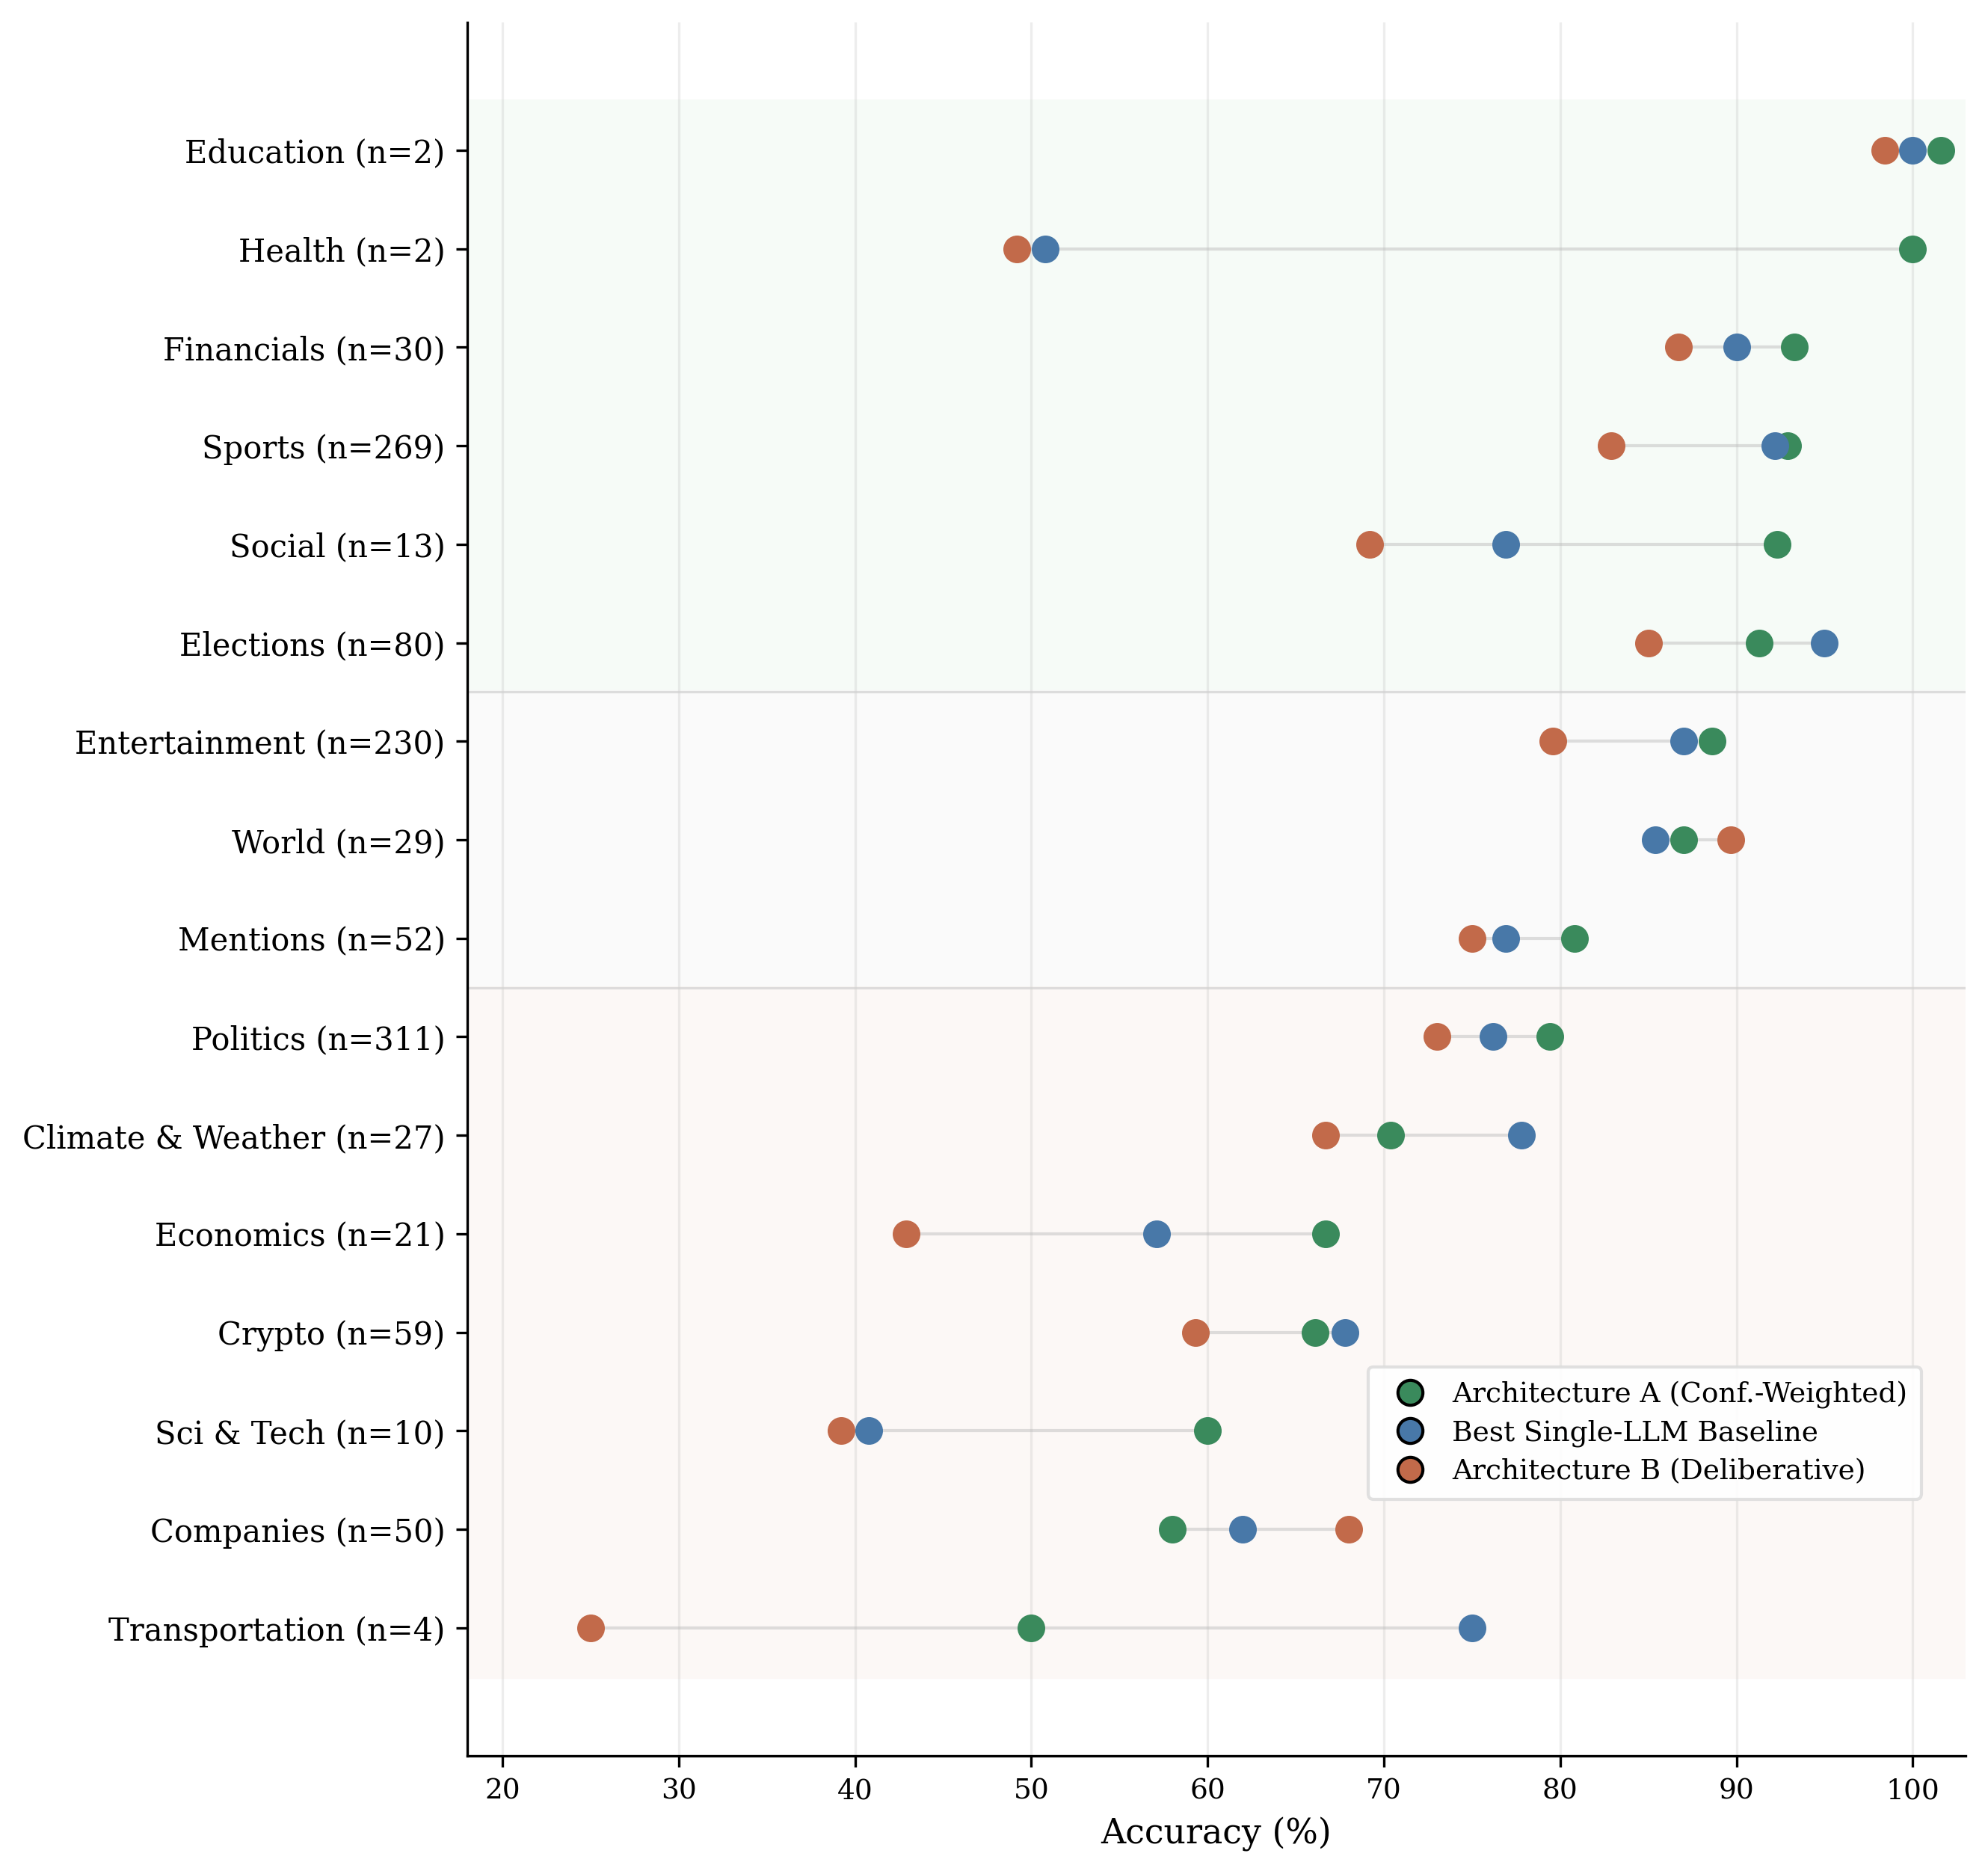
\includegraphics[width=0.65\textwidth]{figures/figure4_category_performance.png}
\caption{\textbf{Category-level accuracy for Architecture A (confidence-weighted), best single-LLM baseline, and Architecture B (deliberative).} Categories are sorted by Architecture A accuracy. Alternating shaded bands delineate the tier structure discussed in the text. Categories with $n < 10$ should be interpreted with caution.}
\label{fig:category_dotplot}
\end{figure}


\begin{table}[t]
\centering
\small
\begin{tabular}{lrccccc}
\toprule
\textbf{Category} & $n$ & \textbf{A Wtd} & \textbf{A Maj} & \textbf{Best Baseline} & \textbf{B Delib} & \textbf{Disagree \%} \\
\midrule
Education           &   2 & 100.0 & 100.0 & 100.0 & 100.0 &  0.0 \\
Health              &   2 & 100.0 & 100.0 &  50.0 &  50.0 & 50.0 \\
Financials          &  30 &  93.3 &  93.3 &  90.0 &  86.7 & 13.3 \\
Sports              & 269 &  92.9 &  91.4 &  92.2 &  82.9 & 13.0 \\
Social              &  13 &  92.3 &  92.3 &  76.9 &  69.2 & 30.8 \\
Elections           &  80 &  91.3 &  91.3 &  95.0 &  85.0 & 13.8 \\
Entertainment       & 230 &  87.8 &  87.8 &  87.8 &  79.6 & 11.7 \\
World               &  29 &  86.2 &  86.2 &  86.2 &  89.7 &  6.9 \\
Mentions            &  52 &  80.8 &  80.8 &  76.9 &  75.0 & 19.2 \\
Politics            & 311 &  79.4 &  79.1 &  76.2 &  73.0 & 24.4 \\
Climate \& Weather  &  27 &  70.4 &  74.1 &  77.8 &  66.7 & 25.9 \\
Economics           &  21 &  66.7 &  66.7 &  57.1 &  42.9 & 28.6 \\
Crypto              &  59 &  66.1 &  62.7 &  67.8 &  59.3 & 18.6 \\
Sci \& Tech         &  10 &  60.0 &  60.0 &  40.0 &  40.0 & 40.0 \\
Companies           &  50 &  58.0 &  58.0 &  62.0 &  68.0 & 20.0 \\
Transportation      &   4 &  50.0 &  50.0 &  75.0 &  25.0 & 75.0 \\
\bottomrule
\end{tabular}
\caption{Accuracy by category for the top-performing systems. $n$ = number of questions per category. A~Wtd = Architecture A confidence-weighted vote. A~Maj = Architecture A majority vote. Best Baseline = highest single-model accuracy in each category. B~Delib = Architecture B deliberative final. Disagree~\% = proportion of questions where at least one of the three models produced a different answer from the other two.}
\label{tab:category}
\end{table}

A clear tier structure emerges across categories. The top tier includes Sports ($n=269$, 92.9\%), Financials ($n=30$, 93.3\%), and Elections ($n=80$, 91.3\%). These are well-covered domains where retrieved evidence tends to be unambiguous and authoritative. In these categories, inter-model disagreement is low (11--14\%), and Architecture A either matches or slightly exceeds the best single-model baseline. This pattern is consistent with Chainlink's findings, which reported 99.7\% accuracy on sports questions where outcomes are well-documented in public sources~\cite{chainlink2025aioracles}. Our somewhat lower sports accuracy (92.9\% vs.\ 99.7\%) may reflect that KalshiBench includes more temporally nuanced sports questions, such as season-level outcomes and conditional events, compared to Chainlink's simpler game-result format.

The middle tier includes Politics ($n=311$, 79.4\%), Mentions ($n=52$, 80.8\%), and Entertainment ($n=230$, 87.8\%). These categories show moderate difficulty with higher disagreement rates (12--24\%). In Politics, which constitutes the largest single category, Architecture A's weighted vote outperforms the best single baseline by 3.2 percentage points (79.4\% vs.\ 76.2\%), suggesting that aggregation provides meaningful benefit precisely when questions involve interpretive ambiguity. This aligns with the theoretical motivation for multi-agent approaches: diverse models are most valuable when no single model reliably dominates.

The bottom tier includes Crypto ($n=59$, 66.1\%), Companies ($n=50$, 58.0\%), and Economics ($n=21$, 66.7\%). These categories exhibit low accuracy across \emph{all} systems, indicating that these failures stem from fundamental difficulty rather than any architecture-specific weakness. Crypto and Companies questions often involve rapidly evolving market conditions, ambiguous resolution criteria (e.g., ``Will token X reach price Y by date Z?''), and thin or contradictory evidence. These are challenges that neither additional models nor deliberation can overcome if the underlying evidence is insufficient. Notably, Companies is the one category where Architecture B (68.0\%) meaningfully outperforms Architecture A (58.0\%), suggesting that deliberation may occasionally help on information-rich questions where models benefit from synthesizing multiple interpretive frames. World events show a similar but smaller pattern (B at 89.7\% vs.\ A at 86.2\%).

One finding that merits caution is Elections. It shows an unusual case where the best single-model baseline (95.0\%) exceeds Architecture A (91.3\%). Manual inspection revealed that one model occasionally held the correct minority position on election questions, and aggregation overrode it. This illustrates a known limitation of majority-rule systems: when one model is systematically better-calibrated on a specific domain, aggregation can dilute its advantage. A potential mitigation would be category-aware weighting, where models receive different influence based on domain-specific track records, though this introduces the risk of overfitting to historical category performance.

Several categories (Education $n=2$, Health $n=2$, Transportation $n=4$, Sci \& Tech $n=10$) have sample sizes too small to draw reliable conclusions. We report their results for completeness but caution against over-interpreting apparent patterns in these categories.

\subsection{Correlated Errors: Why Aggregation Gains Fall Short of the Theoretical Ceiling}
\label{sec:errcorr}

The central promise of multi-agent architectures is that diverse models will make \emph{different} errors, allowing aggregation to filter out individual mistakes. To test this premise, we computed pairwise error correlations and conditional error probabilities across the three oracle agents (Tables~\ref{tab:errcorr} and~\ref{tab:pairwise}).



Error correlations range from moderate to high ($r = 0.529$--$0.689$). GPT-4o exhibits the lowest correlation with the other two models ($r = 0.53$ with Llama, $r = 0.58$ with DeepSeek), making it the most independently-minded oracle agent. DeepSeek and Llama are the most correlated pair ($r = 0.689$), consistent with the hypothesis that open-source models sharing overlapping training data or architectural lineage may inherit similar reasoning blind spots. The conditional error probabilities reinforce this pattern: when DeepSeek is wrong, Llama is also wrong 77.0\% of the time, compared to 63.3\% for GPT-4o when Llama errs.

These correlations have direct implications for the theoretical ceiling of aggregation-based approaches. Under an independence assumption, three models each achieving $\sim$82\% accuracy would be expected to reach approximately 91\% accuracy under majority voting according to the Condorcet Jury Theorem. However, the observed majority-vote accuracy of 82.93\% falls substantially short of this theoretical ceiling. This gap is consistent with the moderate-to-high error correlations observed across models: when one model fails, the others are often failing on the same question for the same underlying reason, typically because the retrieved evidence is ambiguous, incomplete, or misleading.


\begin{table}[t]
\centering
\caption{Pearson correlation of binary error vectors across oracle agents. Higher values indicate models tend to make mistakes on the same questions. A correlation of 1.0 would mean perfectly overlapping errors; 0.0 would mean fully independent error patterns.}
\label{tab:errcorr}
\begin{tabular}{lccc}
\toprule
 & \textbf{GPT-4o} & \textbf{DeepSeek} & \textbf{Llama} \\
\midrule
GPT-4o   & 1.000 & 0.580 & 0.529 \\
DeepSeek & 0.580 & 1.000 & 0.689 \\
Llama    & 0.529 & 0.689 & 1.000 \\
\bottomrule
\end{tabular}
\end{table}


These correlated errors manifest in two ways within our evaluation. First, they explain why Architecture~A's accuracy gains over single-model baselines are modest (+1.01 pp rather than the $\sim$9 pp that independence would predict). Second, they create the conditions under which Architecture~B's deliberation actively degrades performance, a dynamic we analyze as \emph{persuasive error propagation} in Section~\ref{sec:failmode-pep}.


\subsection{Failure Mode Taxonomy}
\label{sec:failure}


The preceding sections quantify accuracy differences across architectures and measure error correlations across models. This section complements those results by analyzing incorrect resolutions to understand why the system fails. We identify five failure modes, four shared across architectures and one specific to Architecture~B's deliberation process.

These failure modes differ primarily in where the error originates. Retrieval failures stem from missing evidence upstream of the resolution pipeline. Temporal reasoning errors arise from misinterpreting the time-relevance of available evidence. Hallucinations involve fabricated claims or criteria interpretations not grounded in the evidence packet. Shared bias reflects correlated misinterpretation of evidence that is present but systematically misread across all models. Finally, persuasive error propagation is unique to Architecture~B, emerging not from individual reasoning but from inter-agent interaction during deliberation.
\begin{table}[t]
\centering
\caption{Conditional error probability: $P(\text{B wrong} \mid \text{A wrong})$. Each cell shows the probability that model B also answers incorrectly, given that model A answered incorrectly. Values above 0.50 indicate positively correlated failure patterns.}
\label{tab:pairwise}
\begin{tabular}{lcc}
\toprule
\textbf{Given A wrong} & \textbf{B = DeepSeek} & \textbf{B = Llama} \\
\midrule
GPT-4o   & 0.652 & 0.633 \\
DeepSeek & ---   & 0.770 \\
Llama    & 0.722 & --- \\
\bottomrule
\end{tabular}
\end{table}

\subsubsection{Retrieval Failure}

A retrieval failure occurs when the evidence packet lacks the information needed to resolve the question correctly, so that agents reach the wrong conclusion despite sound reasoning. The error is upstream of the resolution pipeline, and no amount of multi-agent aggregation or deliberation can compensate.

A representative example is the question (Row 0189) ``If Glen Powell hosts an episode of Saturday Night Live Season 51, then the market resolves to Yes'' (ground truth: YES). The evidence packet contained ten sources listing confirmed SNL Season 51 hosts, but none mentioned Glen Powell. All three agents independently concluded NO, citing his absence from multiple credible host lists. The Exa query returned articles that were either published before Powell's hosting was announced or simply did not mention it, leaving the agents with a systematically incomplete evidence set.

Retrieval failures are particularly difficult to detect at resolution time because the evidence packet appears substantive, agents receive multiple sources, cite them confidently, and produce coherent reasoning chains, yet the critical piece of information is simply absent. This distinguishes retrieval failure from shared bias, where evidence is present but misinterpreted, and from hallucination, where agents fabricate information beyond what the evidence contains.


\subsubsection{Temporal Reasoning Error}

A temporal reasoning error occurs when agents misinterpret the relationship between evidence timestamps and the resolution window, treating the absence of contemporaneous reporting as a negative signal rather than recognizing an evidence gap.

A representative example is the question (Row 0726) ``If the value of the S\&P 500 index value starting Mar 19, 2025 and ending on Jan 1, 2026 is above 6699.99, then the market resolves to Yes'' (ground truth: YES). The evidence packet contained ten sources, all forecasts or projections published in 2023--2024, with none providing actual observed index values from the resolution window. All three agents converged on NO, reasoning that ``forecasts do not count as evidence of an actual crossing.'' This logic is correct in isolation, but the agents conflated two distinct situations: ``the event has not yet occurred'' and ``the event occurred but our evidence does not include post-event reporting.'' The resolution window had already closed and the S\&P~500 had exceeded the threshold, but the evidence packet contained only pre-event forecasts. Rather than expressing appropriate uncertainty, the agents treated the absence of observed data as affirmative evidence that the threshold was never crossed.

This failure mode is particularly insidious because each individual reasoning step is defensible. The error lies in the implicit temporal assumption that if an event had occurred, the evidence packet would contain confirmation. This assumption is violated whenever the retrieval layer returns temporally misaligned sources, a pattern that recurs across Crypto and Financials questions requiring precise price data at specific timestamps.


\subsubsection{Hallucination}

A hallucination occurs when an agent generates claims or interpretations not supported by the evidence packet or resolution criteria, fabricating content that is presented with the same confidence as legitimate reasoning.

A representative example is the question ``If Star appears on Taylor Swift's album `The Life of a Showgirl' before Jan 1, 2026, then the market resolves to Yes'' (ground truth: YES). The resolution criteria specify rules for matching words in lyrics, establishing that the question asks whether the word ``Star'' appears in the album's lyrics. The evidence packet contained multiple sources with titles such as ``Lyrics Revealed'' and ``Lyrics and Track Listing,'' providing extensive lyrical coverage. However, one model reframed the question entirely, interpreting the resolution criterion as asking whether ``a person/entity named `Star' appears on Taylor Swift's album'' as a performer or contributor. From this fabricated premise, the model concluded NO with 0.75 confidence. The other two models similarly concluded NO, reporting that the word ``Star'' was not mentioned across the lyric sources despite the evidence packet containing articles that comprehensively covered the album's lyrics.

This example illustrates two distinct hallucination patterns. The first is criteria fabrication, where the model invents an interpretation of the resolution criteria that diverges from the actual text. The second is negative assertion from incomplete extraction, where models claim a word does not appear in sources whose full content they may not have fully processed. Both patterns produce reasoning grounded in fabricated premises rather than actual evidence.

\subsubsection{Shared Bias}

A shared bias occurs when all three agents independently arrive at the same incorrect answer due to a common interpretive tendency, despite the relevant evidence being present in the packet. Unlike persuasive error propagation, no inter-agent interaction is involved. This failure mode is the direct cause of the correlated errors measured in Section~\ref{sec:errcorr} and explains why majority voting cannot correct a substantial fraction of errors.

A representative example is the question ``If the first budget reconciliation bill to become law before Jan 1, 2027 cuts at least \$800 billion from Medicaid, then the market resolves to Yes'' (ground truth: YES). The evidence packet contained sources estimating approximately \$625 billion in Medicaid cuts under the House bill and indicating the Senate bill would cut over \$200 billion more, implying roughly \$825 billion in total reductions. All three models correctly identified these figures and recognized that the Senate bill would likely exceed the threshold. Yet all three independently concluded NO, applying identical reasoning: because no source explicitly confirmed that a reconciliation bill had been signed into law, the resolution criterion requiring a bill to ``become law'' was not satisfied. Each model treated the absence of explicit enactment confirmation as decisive, despite the evidence strongly suggesting the threshold would be met.

Because this conservative disposition is shared across model families, neither majority voting nor confidence weighting can surface a correct minority opinion. The error is invisible to the aggregation layer precisely because every agent agrees.


\subsubsection{Persuasive Error Propagation}
\label{sec:failmode-pep}

The four failure modes above apply to both architectures. Persuasive error propagation is unique to Architecture~B and represents the mechanism by which deliberation degrades rather than improves accuracy.

\begin{table}[t]
\centering
\caption{Accuracy by convergence stage in Architecture B's deliberative process. Round~1 consensus = all three models agreed after initial independent answers. Round~2 consensus = models converged after viewing each other's reasoning. No consensus = models still disagreed after both rounds. $n$ = number of questions reaching each stage.}
\label{tab:convergence}
\begin{tabular}{lrc}
\toprule
\textbf{Stage} & $n$ & \textbf{Accuracy (\%)} \\
\midrule
Round 1 consensus     & 1,002 & 80.24 \\
Round 2 consensus     &    58 & 56.90 \\
No consensus reached  &   129 & 52.71 \\
\bottomrule
\end{tabular}
\end{table}

Table~\ref{tab:convergence} shows accuracy stratified by when consensus was reached during Architecture~B's deliberative process. The vast majority of questions (84.3\%, $n = 1{,}002$) reached consensus after Round~1 with 80.24\% accuracy, close to the single-model baseline range, since initial agreement essentially reflects that all three models independently arrived at the same answer. The remaining 187 questions (15.7\%) are substantially harder, with accuracy near chance regardless of whether Round~2 deliberation achieved consensus (56.9\%) or not (52.7\%). The marginal difference between these two groups is 4.2 percentage points, which indicates that when models initially disagree on genuinely difficult questions, further debate rarely resolves the disagreement correctly.



To directly measure the effect of deliberation on individual agent decisions, we tracked all revisions between Round~1 and Round~2 of Architecture~B. Of 3{,}567 agent-round pairs, only 88 (2.47\%) resulted in a revision, affecting 83 of 1{,}189 questions (6.98\%). Critically, these revisions were no better than random: 45 flipped a correct answer to incorrect, while 43 flipped an incorrect answer to correct, yielding a net loss of 2 correct predictions. Per-model analysis reveals an asymmetry consistent with the error correlation findings from Section~\ref{sec:errcorr}. GPT-4o, the most independently-minded model with the lowest pairwise error correlations, was the most harmed by deliberation, flipping 26 correct answers to incorrect against only 16 in the opposite direction. DeepSeek, which shares the highest error correlation with Llama ($r = 0.689$), was the only model to benefit from revisions (3 correct-to-incorrect versus 9 incorrect-to-correct). This pattern suggests that the most independent model is disproportionately vulnerable to being talked out of correct minority positions by a correlated majority, precisely the dynamic that undermines the theoretical promise of multi-agent deliberation. Figure~\ref{fig:revision_flows} visualizes these revision flows for each model.

The mechanism behind this failure appears to be what we term \emph{persuasive error propagation}. During deliberation, a model that is confidently wrong can present compelling but flawed reasoning that causes a correct model to revise its answer. Because the questions where models initially disagree are precisely the ambiguous ones where evidence supports multiple interpretations, a well-articulated wrong argument is often indistinguishable from a right one. This dynamic is the opposite of what Du et al.~\cite{du2023debate} observed in arithmetic tasks, where correct reasoning is verifiable step-by-step and errors are easy to identify during debate. Oracle resolution lacks this verifiability: the correct interpretation of ambiguous evidence cannot be derived through logic alone, making deliberation vulnerable to confident miscalibration.

\begin{figure}[t]
\centering
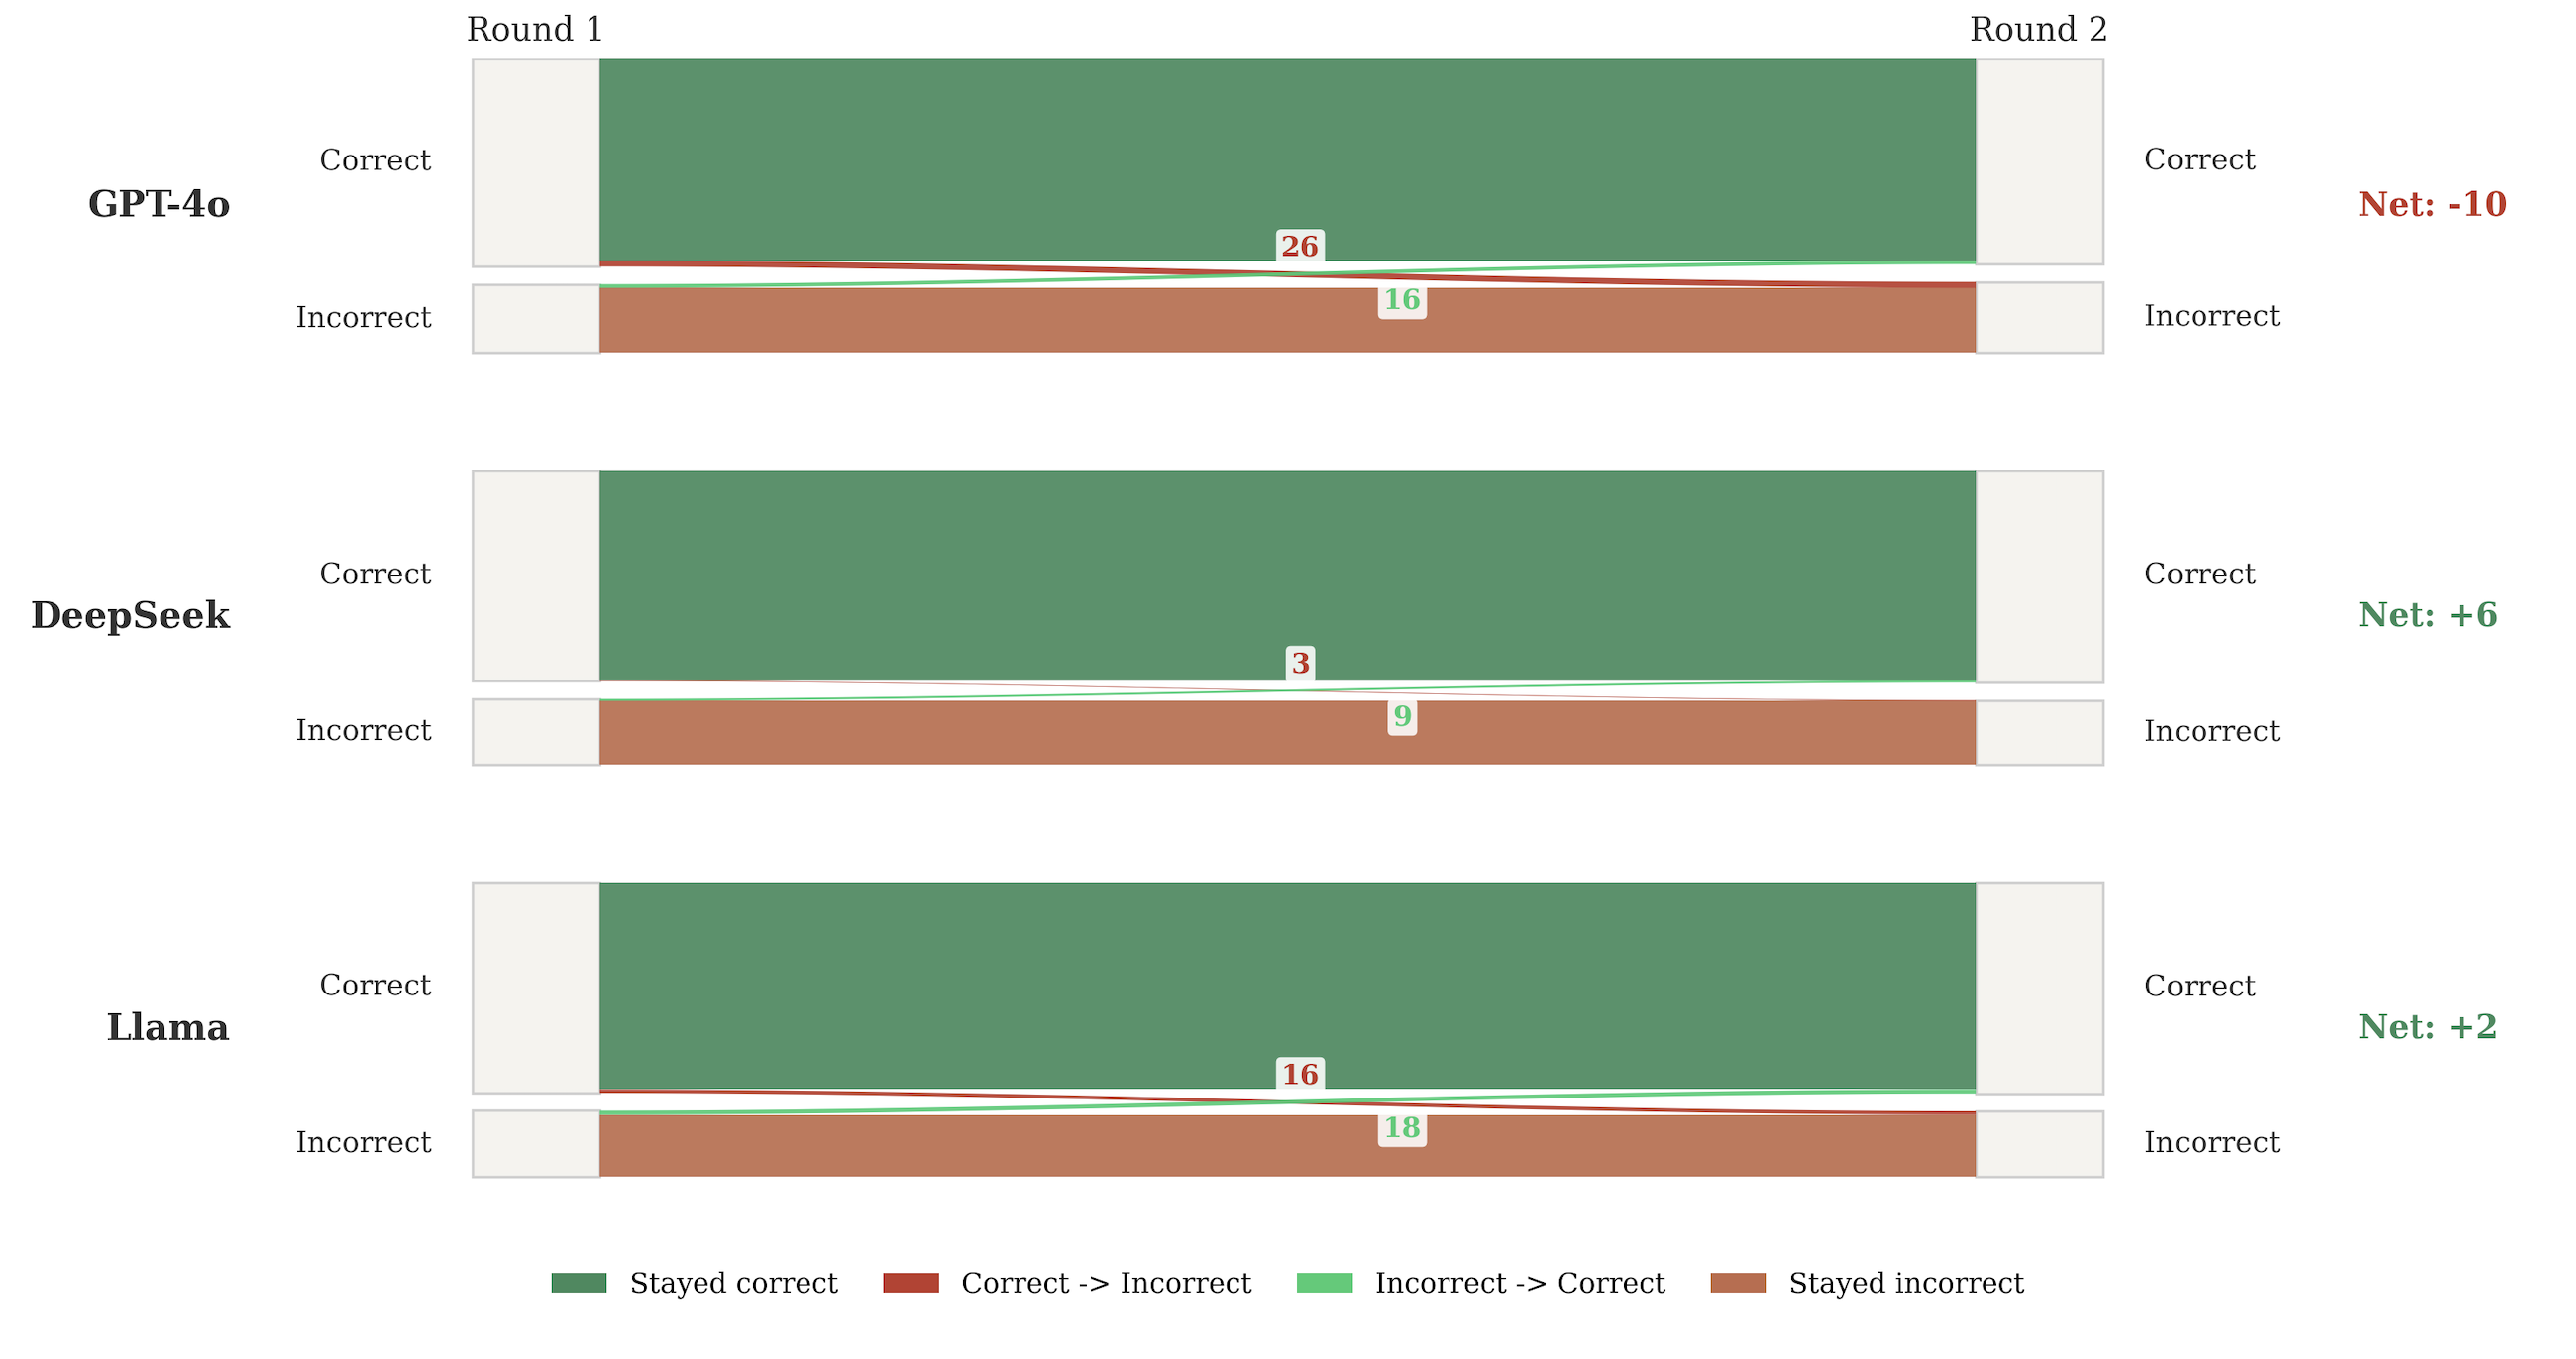
\includegraphics[width=0.75\textwidth]{figures/figure5_debate_transition_analysis.png}
\caption{\textbf{Answer revision flows between Round~1 and Round~2 in Architecture~B.} Red indicates correct-to-incorrect flips, and green indicates incorrect-to-correct flips. Deliberation yields a net loss in accuracy for GPT-4o (--10) and gains for DeepSeek (+6).}
\label{fig:revision_flows}
\end{figure}

This finding carries practical design implications. For oracle systems where fast, reliable resolution is the priority, independent aggregation with confidence weighting is both simpler and more accurate than deliberation. Deliberation's computational cost, which requires multiple rounds of inference with full context windows containing other models' reasoning, is not justified by improved accuracy. If anything, the additional expense buys worse outcomes. The one exception, as noted in Section~\ref{sec:category}, is that deliberation occasionally helps on information-dense categories like Companies and World events, where synthesizing multiple interpretive perspectives may add genuine value. A potential hybrid design could route questions through independent aggregation by default, reserving deliberation only for categories where it has demonstrated benefit. This would require sufficient category-level data to calibrate routing decisions reliably.

\subsection{Escalation Criteria for Hybrid Oracle Systems}
\label{sec:escalation}
 
In a deployed oracle system, auto-resolving all questions with Architecture~A yields 82.93\% accuracy. While this represents a meaningful improvement over single-model baselines, the remaining 17\% error rate is substantial for a system settling financial contracts. Human arbitration can achieve higher accuracy but at significant cost and latency. UMA's dispute resolution mechanism requires 48 to 96 hours and involves token-holder voting, while Kalshi's internal operations team provides reliable resolution but is extremely time intensive when scaled to thousands of simultaneous markets. A practical hybrid system needs principled routing rules that auto-resolve high-confidence questions while escalating uncertain ones to human review.
 
We find that inter-agent agreement is the single strongest predictor of resolution accuracy in Architecture~A. Table~\ref{tab:agreement_status} shows accuracy stratified by agreement status across all 1,189 questions. When all three models independently produce the same answer, accuracy reaches 88.34\%. When the vote splits 2-1, accuracy drops to 57.82\%, barely above chance for a binary task. This 30.5 percentage point gap demonstrates that disagreement among independently reasoning models is a highly informative signal that a question is likely to be resolved incorrectly.
 
\begin{table}[h]
\centering
\caption{Architecture~A resolution accuracy by inter-agent agreement status across all 1,189 questions. Unanimous indicates all three models produced the same binary decision; Split indicates a 2-1 vote.}
\label{tab:agreement_status}
\begin{tabular}{lcc}
\hline
Agreement Status & $n$ & Accuracy (\%) \\
\hline
Unanimous (3-0) & 978 & 88.34 \\
Split (2-1) & 211 & 57.82 \\
\hline
\end{tabular}
\end{table}
 
Average model confidence provides additional discriminative power, particularly within the unanimous group. Table~\ref{tab:signal_2x2} combines agreement status with confidence, splitting questions at the median average confidence of 0.91. The unanimous and high-confidence cell achieves 97.87\% accuracy on 563 questions, representing the system's most reliable operating regime. Within unanimous questions, confidence separates near-perfect resolution (97.87\%) from substantially weaker performance (75.42\%). However, for split questions, confidence provides almost no additional signal: accuracy is 56.52\% for high-confidence splits and 58.18\% for low-confidence splits. This asymmetry indicates that agreement is the primary escalation signal, with confidence serving as a useful refinement only when models agree.
 
\begin{table}[h]
\centering
\caption{Architecture~A resolution accuracy by combined agreement status and average confidence. Confidence is split at the median average confidence score (0.91) across all 1,189 questions.}
\label{tab:signal_2x2}
\begin{tabular}{lcccc}
\hline
 & \multicolumn{2}{c}{High Confidence} & \multicolumn{2}{c}{Low Confidence} \\
 & $n$ & Accuracy (\%) & $n$ & Accuracy (\%) \\
\hline
Unanimous & 563 & 97.87 & 415 & 75.42 \\
Split & 46 & 56.52 & 165 & 58.18 \\
\hline
\end{tabular}
\end{table}
 
Figure~\ref{fig:coverage_accuracy} presents the coverage-accuracy tradeoff curve for both architectures, constructed by ranking questions in descending order of composite escalation score and computing cumulative accuracy as coverage expands. Architecture~A achieves 100\% accuracy when auto-resolving only the top 10\% of questions, 97.47\% at 50\% coverage, and 90.12\% at 75\% coverage. Architecture~A dominates Architecture~B across most of the operating range, with the gap reaching 10.44 percentage points at 50\% coverage. Architecture~B is marginally better at the extreme top of the ranking (100\% vs.\ 99.15\% at 10\% coverage), but this advantage disappears by 20\% coverage and Architecture~A is consistently superior thereafter.
 
\begin{figure}[h]
\centering
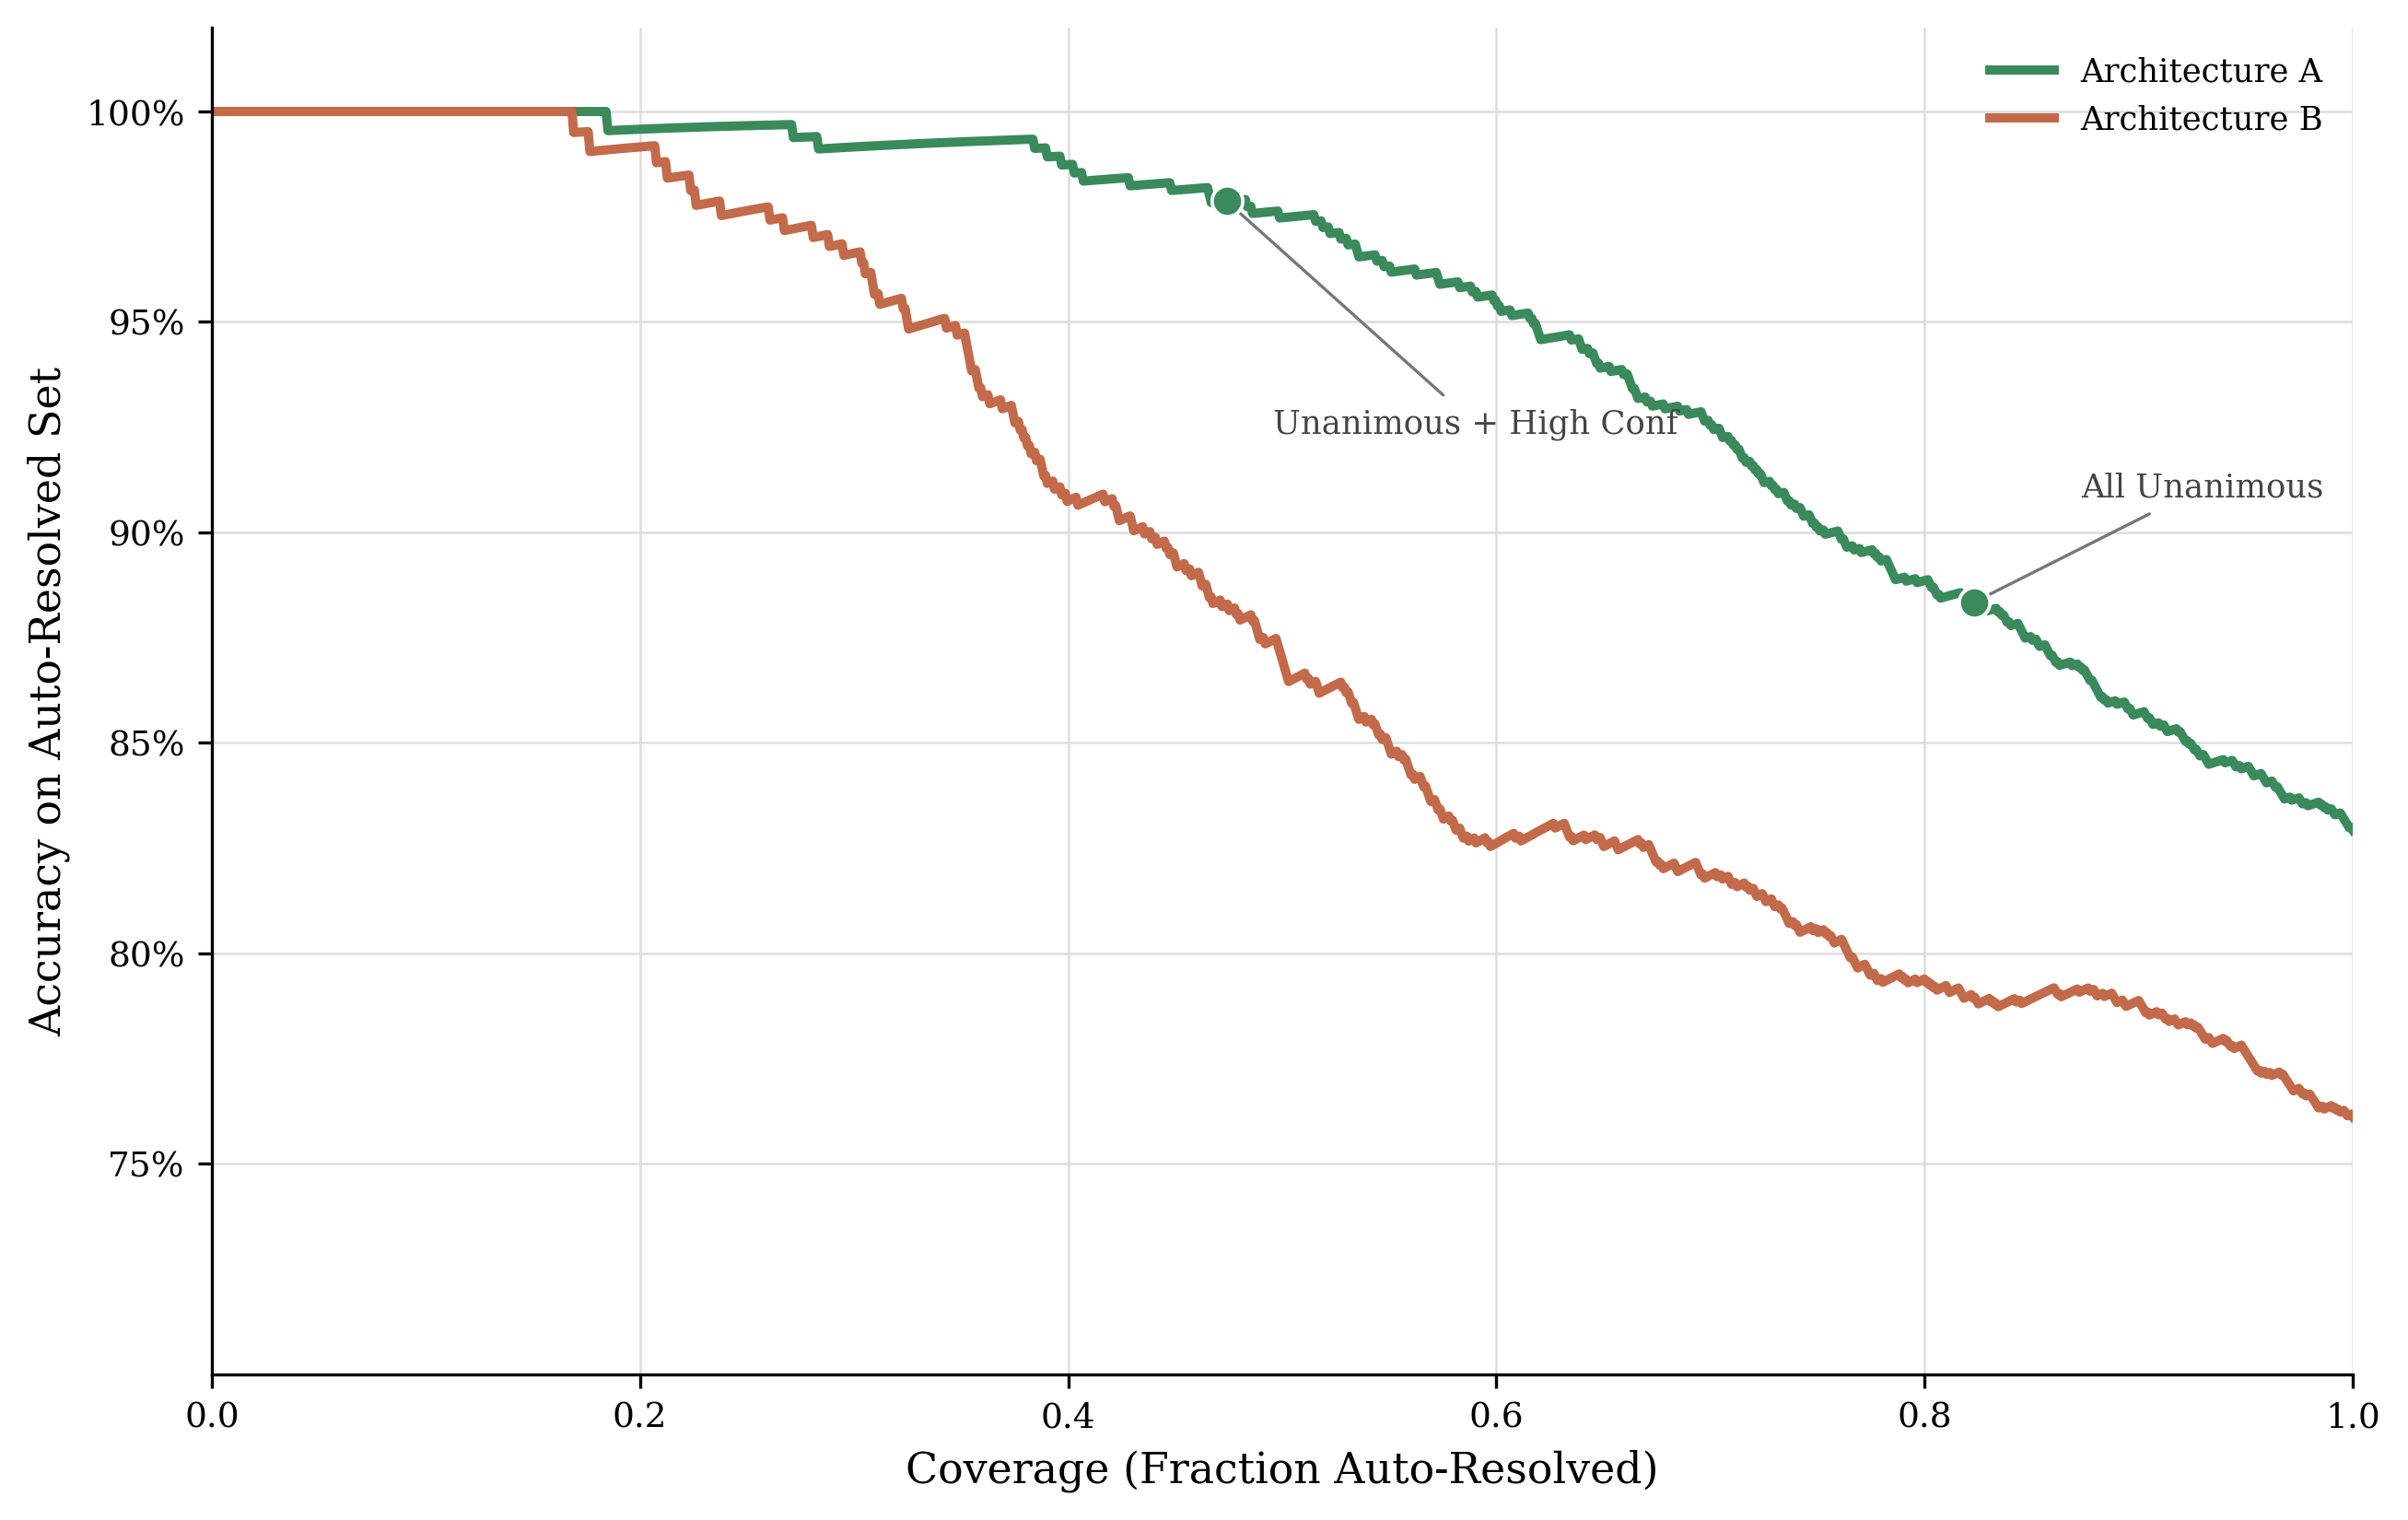
\includegraphics[width=\textwidth]{figures/figure6_escalation_tradeoff_curve.png}
\caption{\textbf{Coverage-accuracy tradeoff curves for Architecture~A and Architecture~B}. Each point represents the cumulative accuracy when auto-resolving the top $k$ questions ranked by composite escalation score. Architecture~A dominates across most of the operating range.}
\label{fig:coverage_accuracy}
\end{figure}
 
These results suggest a practical escalation policy for deployed oracle systems. If a system auto-resolves only unanimous, high-confidence questions, it covers 47.4\% of the dataset at 97.87\% accuracy, escalating the remaining 52.6\% to human arbitration. Relaxing the threshold to include all unanimous questions regardless of confidence increases coverage to 82.3\% at 88.34\% accuracy. An oracle designer can select a point on the coverage-accuracy curve that matches their accuracy tolerance and arbitration budget. For context, at 50\% coverage Architecture~A approaches the accuracy levels that Chainlink reported for sports questions (99.7\%) while handling a much broader range of question categories.
 
This analysis treats escalation as a post-hoc empirical investigation rather than a trained decision system. Formal learning-to-defer approaches jointly optimize a classifier and a rejection function to maximize system-level performance \cite{mozannar2020consistent}. Recent work \cite{jung2025trust} has extended this to cascaded LLM systems with provable guarantees of human agreement at user-specified risk tolerances. Applying these formal frameworks to oracle resolution, where the deferral target is human arbitration with known cost and accuracy characteristics, represents a natural direction for future work.
